\documentclass[a4paper,12pt]{article}
\usepackage{ucs}
\usepackage[utf8x]{inputenc}
\usepackage{amsfonts}
\usepackage[english,russian]{babel}
\usepackage[T1,T2A]{fontenc}
\frenchspacing
\usepackage{amsmath,amssymb,amsthm}
\usepackage[a4paper, margin=1in]{geometry}
\usepackage[table]{xcolor}
\usepackage{multirow}
\usepackage{diagbox}
\usepackage{graphicx}
\graphicspath{ {./} }

\newtheorem{name}{Printed output}
\newtheorem{problem}{Задача}
\newenvironment{solution}{\renewcommand{\proofname}{\unskip\indent\nopunct}\begin{proof}}{\end{proof}}

\begin{document}

\title{ДЗ 6}
\author{Витя\,Ефремов}
\maketitle

\begin{problem}
Задана дискретная двумерная случайная величина (X, Y):
\begin{table}[h!]
\centering
\begin{tabular}{|c|c|c|c|}
    \hline
    \multicolumn{2}{|c|}{} & \multicolumn{2}{c|}{X} \\ \cline{3-4}
    \multicolumn{2}{|c|}{} & 3 & 6 \\ \hline
    \multirow{3}{*}{Y} & 10 & 0.25 & 0.10 \\ \cline{2-4}
    & 14 & 0.15 & 0.05 \\ \cline{2-4}
    & 18 & 0.32 & 0.13 \\ \hline
\end{tabular}
\caption{Совместное распределение}
\end{table}

\begin{enumerate}
    \item Найти коэффициент корреляции.
    \item Построить совместную функцию распределения.
    \item Найти условное среднее $E(Y | X)$.
\end{enumerate}

\end{problem}


\begin{solution}

Маргинальные вероятности:
\begin{table}[h!]
    \centering
    \begin{tabular}{|c|c|c|}
        \hline
        $X$ & 3 & 6 \\
        \hline
        $p_X$ & 0.72 & 0.28 \\
        \hline
    \end{tabular}
    \quad
    \begin{tabular}{|c|c|c|c|}
        \hline
        $Y$ & 10 & 14 & 18 \\
        \hline
        $p_Y$ & 0.35 & 0.2 & 0.45 \\
        \hline
    \end{tabular}
    \caption{Маргинальные распрееления}
\end{table}

Коэффициент корреляции выражается через ковариацию и среднеквадратичные отклонения.
Ковариация, в свою очередь, ищется через матожидания случайных величин $X, Y, X \cdot Y$.
\begin{align*}
    \rho_{X, Y} &= \frac{cov(X, Y)}{\sigma_X \sigma_Y} \\
    cov(X, Y) &= \mathbb E[(X - \mu_X)(Y - \mu_Y)] = \mu_{XY} - \mu_X \mu_Y \\
\end{align*}

Найдем ковариацию:
\begin{align*}
    \mu_X &= \mathbb EX = 3 \cdot 0.72 + 6 \cdot 0.28 = 3.84 \\
    \mu_Y &= \mathbb EY = 10 \cdot 0.35 + 14 \cdot 0.2 + 18 \cdot 0.45 = 14.4 \\
    \mu_{XY} &= \mathbb E[XY] = 3 \cdot 10 \cdot 0.25 + 3 \cdot 14 \cdot 0.15 + 3 \cdot 18 \cdot 0.32 + 6 \cdot 10 \cdot 0.1 + \\
    & + 6 \cdot 14 \cdot 0.05 + 6 \cdot 18 \cdot 0.13 = 55.32 \\
    cov(X, Y) &= \mathbb E[(X - \mu_X)(Y - \mu_Y)] = \mu_{XY} - \mu_X \mu_Y = 55.32 - 3.84 \cdot 14.4 = 0.024 \\
\end{align*}

Найдем СКО:
\begin{align*}
    \sigma^2_X &= \mathbb E[X^2] - \mu_X^2 = 3^2 \cdot 0.72 + 6^2 \cdot 0.28 - 3.84^2 = 16.56 - 14.7456 = 1.8144 \\
    \sigma_X &= \sqrt{1.8144} \approx 1.34699665924 \\
    \sigma^2_Y &= \mathbb E[Y^2] - \mu_Y^2 = 10^2 \cdot 0.35 + 14^2 \cdot 0.2 + 18^2 \cdot 0.45 - 14.4^2 = 220 - 207.36 = 12.64 \\
    \sigma_Y &= \sqrt{12.64} \approx 3.55527776693 \\
\end{align*}
Итого, коэффициент корреляции:
\[
    \rho_{X, Y} = \frac{cov(X, Y)}{\sigma_X \sigma_Y} \approx \frac{0.024}{1.34699665924 \cdot 3.55527776693} \approx \pmb{0.005} \\
\]

Совместная функция распределения получается из таблицы распределения суммированием всех ячеек левее и выше:

\begin{table}[h!]
    \centering
    \begin{tabular}{|c|c|c|c|c|}
        \hline
        \multicolumn{2}{|c|}{} & \multicolumn{3}{c|}{X} \\
        \cline{3-5}
        \multicolumn{2}{|c|}{} & $X<3$ & $3 \le X<6$ & $6 \le X$ \\
        \hline
        \multirow{3}{*}{Y} & $Y<10$    & 0 & 0 & 0 \\ \cline{2-5}
                           & $10 \le Y<14$ & 0 & 0.25 & 0.35 \\ \cline{2-5}
                           & $14 \le Y<18$ & 0 & 0.4 & 0.55 \\ \cline{2-5}
                           & $18 \le Y$    & 0 & 0.87 & 1 \\
        \hline
    \end{tabular}
    \caption{Совместная функция распределения}
\end{table}

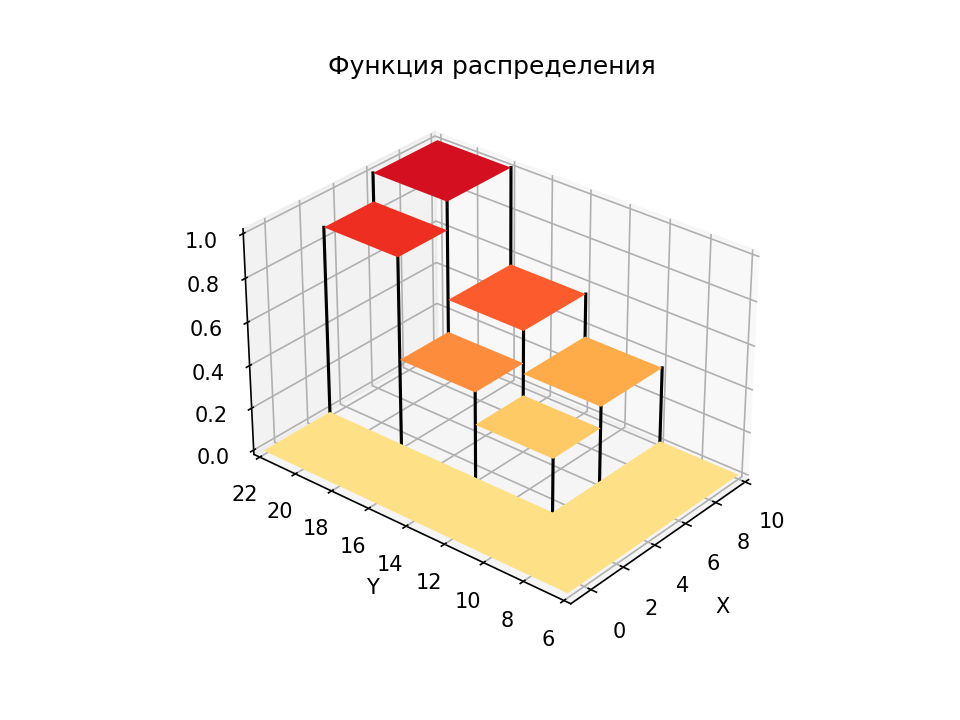
\includegraphics[width=\textwidth]{hw_6.png}

Условное матожидание $\mathbb E(Y | X)$ можно мыслить как функцию от $X$.
Например, при $X=3$ двумерня случайная величина становится одномерной, матожидание этой одномерной случайной величины (число) -- значение условного среднего, при условии $X=3$.

Значение условного матожидания при каждом фиксированном $x$ вычисляется по формулам (обратим внимание, что в первой сумме вероятности условные, а во второй -- совместные):
\[
    \mathbb E(Y | X = x) = \sum_y y \cdot p(Y = y | X = x) = \sum_y y \cdot \frac{p(Y = y, X = x)}{p(X = x)}
\]
\begin{align*}
    \mathbb E(Y | X = 3) &= \frac{10 \cdot 0.25 + 14 \cdot 0.15 + 18 \cdot 0.32}{0.72} = 14.3888888889 \\
    \mathbb E(Y | X = 6) &= \frac{10 \cdot 0.1 + 14 \cdot 0.05 + 18 \cdot 0.13}{0.28} = 14.4285714286 \\
\end{align*}

\end{solution}
\end{document}
